\documentclass[11pt,a4paper]{article}
\usepackage[T1]{fontenc}
\usepackage[utf8]{inputenc}
\usepackage{lmodern}
\usepackage{microtype}
\usepackage[a4paper,margin=21mm,headheight=15pt]{geometry}
\usepackage[table]{xcolor}
\usepackage{booktabs,tabularx,longtable,array}
\usepackage{amsmath,graphicx}
\usepackage{tikz}
\usepackage{fancyhdr}
\usepackage{enumitem}
\usepackage{listings}
\usepackage{titlesec}
\usepackage[hidelinks]{hyperref}
\usetikzlibrary{arrows.meta,positioning,calc,fit,backgrounds}

\definecolor{YTwoBlue}{HTML}{2563EB}
\definecolor{YTwoCyan}{HTML}{0891B2}
\definecolor{YTwoGreen}{HTML}{059669}
\definecolor{YTwoAmber}{HTML}{D97706}
\definecolor{YTwoRed}{HTML}{DC2626}
\definecolor{YTwoPurple}{HTML}{7C3AED}
\definecolor{YTwoInk}{HTML}{172033}
\definecolor{YTwoMuted}{HTML}{5F6B7A}
\definecolor{YTwoPaper}{HTML}{F5F7FA}
\definecolor{YTwoLine}{HTML}{D8DEE8}

\hypersetup{
  colorlinks=true,
  linkcolor=YTwoBlue,
  urlcolor=YTwoBlue,
  pdftitle={Youtube2knowledge: de video a conocimiento verificable},
  pdfauthor={Alberto Muñoz}
}
\pagestyle{fancy}
\fancyhf{}
\lhead{Youtube2knowledge}
\rhead{Whitepaper técnico}
\cfoot{\thepage}
\renewcommand{\headrulewidth}{0.4pt}
\titleformat{\section}{\sffamily\Large\bfseries\color{YTwoInk}}{\thesection}{0.7em}{}
\titleformat{\subsection}{\sffamily\large\bfseries\color{YTwoBlue}}{\thesubsection}{0.7em}{}
\titleformat{\subsubsection}{\sffamily\normalsize\bfseries\color{YTwoPurple}}{\thesubsubsection}{0.7em}{}
\setlength{\parindent}{0pt}
\setlength{\parskip}{0.62em}
\renewcommand{\arraystretch}{1.18}
\setlist[itemize]{leftmargin=5mm,itemsep=2pt,topsep=3pt}
\setlist[enumerate]{leftmargin=6mm,itemsep=2pt,topsep=3pt}
\renewcommand{\figurename}{Figura}
\renewcommand{\tablename}{Tabla}
\renewcommand{\contentsname}{Contenido}

\lstdefinestyle{y2k}{
  basicstyle=\ttfamily\small,
  backgroundcolor=\color{YTwoPaper},
  frame=single,
  rulecolor=\color{YTwoLine},
  breaklines=true,
  columns=fullflexible,
  keepspaces=true,
  showstringspaces=false,
  keywordstyle=\color{YTwoBlue}\bfseries,
  commentstyle=\color{YTwoMuted},
  stringstyle=\color{YTwoGreen},
  xleftmargin=3mm,
  xrightmargin=3mm
}
\lstset{style=y2k}

\newcommand{\pill}[2]{%
  \tikz[baseline=(n.base)]\node[
    fill=#1!12,draw=#1!55,rounded corners=1.5mm,
    inner xsep=2.4mm,inner ysep=1mm,
    font=\sffamily\scriptsize\bfseries,text=#1
  ] (n) {#2};%
}

\begin{document}
\hypersetup{pageanchor=false}
\begin{titlepage}
  \thispagestyle{empty}
  \color{YTwoInk}
  \vspace*{18mm}
  {\sffamily\bfseries\fontsize{35}{40}\selectfont Youtube2knowledge\par}
  \vspace{4mm}
  {\sffamily\fontsize{20}{25}\selectfont De video a conocimiento verificable\par}
  \vspace{9mm}
  {\sffamily\large\color{YTwoMuted}
    Arquitectura, modelos locales, resolución de incidentes y despliegue\par}
  \vspace{15mm}
  
\begin{tikzpicture}
    \fill[YTwoBlue] (0,0) rectangle (3.4,0.18);
    \fill[YTwoCyan] (3.4,0) rectangle (6.6,0.18);
    \fill[YTwoPurple] (6.6,0) rectangle (10.1,0.18);
    \fill[YTwoGreen] (10.1,0) rectangle (15.3,0.18);
  \end{tikzpicture}
  \vspace{17mm}

  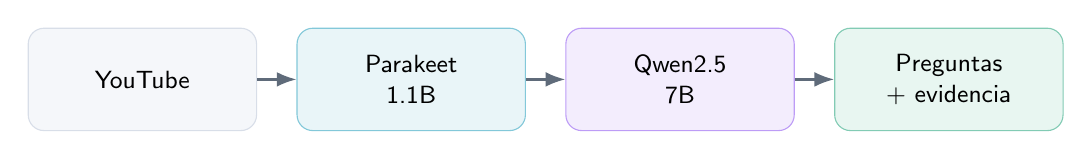
\begin{tikzpicture}[
    node distance=5mm,
    stage/.style={draw=YTwoLine,rounded corners=2mm,minimum width=29mm,
      minimum height=13mm,align=center,fill=YTwoPaper,font=\sffamily\small},
    arrow/.style={-{Latex[length=2.5mm]},line width=0.8pt,draw=YTwoMuted}
  ]
    \node[stage] (video) {YouTube};
    \node[stage,right=of video,fill=YTwoCyan!9,draw=YTwoCyan!50] (asr)
      {Parakeet\\1.1B};
    \node[stage,right=of asr,fill=YTwoPurple!9,draw=YTwoPurple!50] (llm)
      {Qwen2.5\\7B};
    \node[stage,right=of llm,fill=YTwoGreen!9,draw=YTwoGreen!50] (knowledge)
      {Preguntas\\+ evidencia};
    \draw[arrow] (video) -- (asr);
    \draw[arrow] (asr) -- (llm);
    \draw[arrow] (llm) -- (knowledge);
  \end{tikzpicture}

  \vfill
  {\sffamily\large Alberto Muñoz\par}
  {\sffamily\color{YTwoMuted}NVIDIA DGX Spark GB10\par}
  {\sffamily\color{YTwoMuted}2 de septiembre de 2026\par}
  \vspace{5mm}
  {\sffamily\small
    \href{https://youtube2knowledge-five.vercel.app/}{youtube2knowledge-five.vercel.app}\par}
  {\sffamily\small
    \href{https://github.com/LuisAlbertoMunozUbando/youtube2knowledge}
    {github.com/LuisAlbertoMunozUbando/youtube2knowledge}\par}
\end{titlepage}

\pagenumbering{roman}
\hypersetup{pageanchor=true}
\section*{Resumen ejecutivo}
\addcontentsline{toc}{section}{Resumen ejecutivo}

Youtube2knowledge convierte un video público de YouTube en un paquete de
conocimiento trazable. El sistema extrae y normaliza el audio, lo transcribe con
NVIDIA Parakeet 1.1B RNNT Multilingual, usa Qwen2.5-7B-Instruct para formular
preguntas educativas y respuestas, valida cada evidencia contra la transcripción
y archiva el resultado completo en Google Drive.

La solución separa la experiencia web de la carga de cómputo. Next.js se publica
en Vercel; Cloudflare Tunnel conecta el navegador con FastAPI en una NVIDIA DGX
Spark; los modelos, las claves y los datos persistentes permanecen locales.

El desarrollo exigió resolver autenticación NGC, selección del perfil GB10,
permisos del caché NIM, DNS dentro del contenedor, descarga Xet, parseo de CORS,
formato de audio, alineación de evidencia, sincronización de Drive y dos fallos
independientes de Vercel. El documento conserva la arquitectura final y el
razonamiento diagnóstico que permitió llegar a ella.

\vspace{5mm}
\begin{center}
  \pill{YTwoGreen}{DESPLIEGUE WEB EXITOSO}\quad
  \pill{YTwoBlue}{ASR VALIDADO}\quad
  \pill{YTwoPurple}{LLM VALIDADO}\quad
  \pill{YTwoAmber}{ARCHIVO DRIVE}
\end{center}

\clearpage
\tableofcontents
\clearpage
\hypersetup{pageanchor=false}
\pagenumbering{arabic}
\hypersetup{pageanchor=true}

\section{Visión del producto}

El video es sencillo de consumir, pero difícil de consultar, verificar y
reutilizar. Una transcripción aislada tampoco basta: el usuario necesita preguntas
relevantes, respuestas breves y un camino de regreso a la evidencia.

Youtube2knowledge permite seleccionar \emph{What, Which, Where, When, How, Why,
Who} y \emph{Whose}, añadir palabras clave, escribir preguntas propias, elegir el
idioma y fijar cuántas preguntas se generan por tipo.

\subsection{Principios}
\begin{itemize}
  \item \textbf{Evidencia antes que elocuencia:} es mejor omitir que inventar.
  \item \textbf{IA local:} ASR y LLM se ejecutan en la DGX Spark.
  \item \textbf{Responsabilidades separadas:} web, edge, API, modelos y archivo.
  \item \textbf{Recuperación incremental:} un fallo del LLM no repite el ASR.
  \item \textbf{Estado durable:} jobs y resultados sobreviven recargas y reinicios.
\end{itemize}

\section{Arquitectura}

\begin{figure}[htbp]
  \centering
  \resizebox{\textwidth}{!}{%
  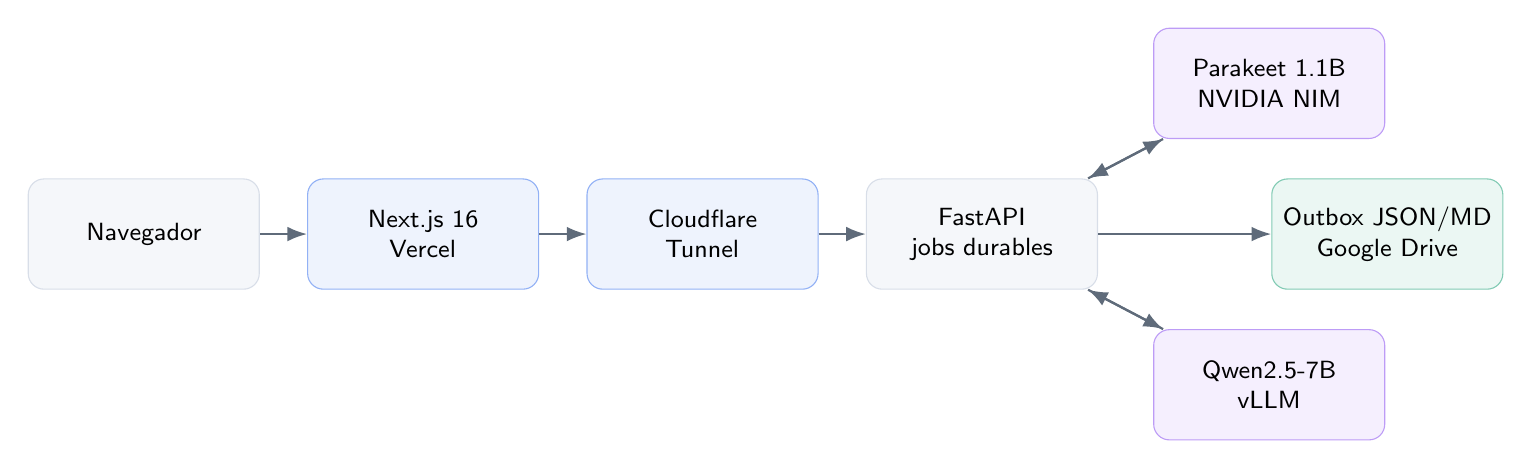
\begin{tikzpicture}[
    node distance=6mm,
    box/.style={draw=YTwoLine,rounded corners=2mm,minimum height=14mm,
      text width=27mm,align=center,fill=YTwoPaper,font=\sffamily\small},
    web/.style={box,fill=YTwoBlue!8,draw=YTwoBlue!50},
    gpu/.style={box,fill=YTwoPurple!8,draw=YTwoPurple!50},
    data/.style={box,fill=YTwoGreen!8,draw=YTwoGreen!50},
    arrow/.style={-{Latex[length=2.5mm]},line width=0.8pt,draw=YTwoMuted}
  ]
    \node[box] (browser) {Navegador};
    \node[web,right=of browser] (vercel) {Next.js 16\\Vercel};
    \node[web,right=of vercel] (cf) {Cloudflare\\Tunnel};
    \node[box,right=of cf] (api) {FastAPI\\jobs durables};
    \node[gpu,above right=5mm and 7mm of api] (asr) {Parakeet 1.1B\\NVIDIA NIM};
    \node[gpu,below right=5mm and 7mm of api] (llm) {Qwen2.5-7B\\vLLM};
    \node[data,right=22mm of api] (drive) {Outbox JSON/MD\\Google Drive};
    \draw[arrow] (browser) -- (vercel);
    \draw[arrow] (vercel) -- (cf);
    \draw[arrow] (cf) -- (api);
    \draw[arrow] (api) -- (asr);
    \draw[arrow] (asr) -- (api);
    \draw[arrow] (api) -- (llm);
    \draw[arrow] (llm) -- (api);
    \draw[arrow] (api) -- (drive);
  \end{tikzpicture}}
  \caption{Arquitectura de producción: web pública y cómputo local desacoplados.}
\end{figure}

\begin{tabularx}{\textwidth}{@{}l X X@{}}
  \toprule
  Frontera & Expuesto & Protegido \\
  \midrule
  Vercel & HTML, CSS y JavaScript & Ninguna clave de modelo \\
  Cloudflare & Host HTTPS de la API & IP y puertos internos \\
  FastAPI & Salud y jobs & Validación, límites y estado \\
  DGX Spark & Puerto 8020 por túnel & ASR 9000 y LLM 8001 en loopback \\
  Google Drive & Carpeta de resultados & rclone montado sólo lectura \\
  \bottomrule
\end{tabularx}

\subsection{Estados del pipeline}

\begin{figure}[htbp]
  \centering
  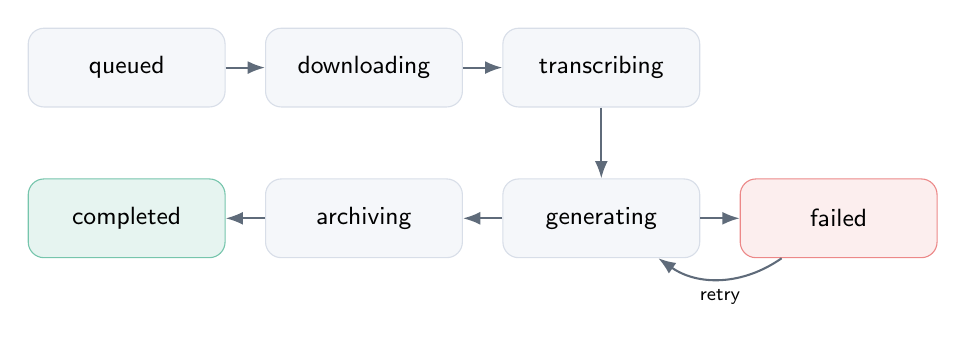
\begin{tikzpicture}[
    node distance=5mm,
    state/.style={draw=YTwoLine,rounded corners=2mm,minimum width=25mm,
      minimum height=10mm,align=center,fill=YTwoPaper,font=\sffamily\small},
    arrow/.style={-{Latex[length=2.2mm]},line width=0.75pt,draw=YTwoMuted}
  ]
    \node[state] (q) {queued};
    \node[state,right=of q] (d) {downloading};
    \node[state,right=of d] (t) {transcribing};
    \node[state,below=9mm of t] (g) {generating};
    \node[state,left=of g] (a) {archiving};
    \node[state,left=of a,fill=YTwoGreen!10,draw=YTwoGreen!55] (c) {completed};
    \node[state,right=of g,fill=YTwoRed!8,draw=YTwoRed!55] (f) {failed};
    \draw[arrow] (q)--(d);\draw[arrow] (d)--(t);\draw[arrow] (t)--(g);
    \draw[arrow] (g)--(a);\draw[arrow] (a)--(c);\draw[arrow] (g)--(f);
    \draw[arrow,bend left=35] (f) to node[below,font=\sffamily\scriptsize]{retry} (g);
  \end{tikzpicture}
  \caption{Máquina de estados persistente y reintento sólo de generación.}
\end{figure}

\section{Plataforma NVIDIA DGX Spark}

La máquina objetivo usa arquitectura \texttt{aarch64}, GPU NVIDIA GB10, driver
580.159.03, CUDA 13.0 y Docker Compose 5.0.2. Durante la puesta en marcha había
121 GiB de memoria y 2.7 TiB libres.

\begin{table}[htbp]
  \centering
  \caption{Servicios del despliegue Spark.}
  \begin{tabularx}{\textwidth}{@{}l l l X@{}}
    \toprule
    Servicio & Puerto host & Cómputo & Función \\
    \midrule
    \texttt{asr} & 127.0.0.1:9000 & GPU & Speech NIM con Parakeet \\
    \texttt{llm} & 127.0.0.1:8001 & GPU & vLLM con Qwen2.5-7B \\
    \texttt{api} & 0.0.0.0:8020 & CPU & FastAPI y jobs \\
    \texttt{drive-sync} & sin puerto & CPU & Copia mediante rclone \\
    \bottomrule
  \end{tabularx}
\end{table}

\section{Pipeline de conocimiento}

\subsection{Ingesta y audio}
La API sólo acepta videos individuales de \texttt{youtube.com} y
\texttt{youtu.be}. \texttt{yt-dlp} obtiene metadatos y el mejor audio. FFmpeg
normaliza a WAV PCM de 16 bits, mono y 16 kHz:

\begin{lstlisting}[language=bash]
ffmpeg -i source -vn -ac 1 -ar 16000 -c:a pcm_s16le audio.wav
\end{lstlisting}

Los audios grandes se dividen para mantener cada petición por debajo de 20 MiB.

\subsection{Transcripción}
Parakeet usa el perfil offline multilingüe de DGX Spark con VAD Silero y
diarización Sortformer. La API envía \texttt{language=multi} para detección
automática y habilita puntuación.

\subsection{Preguntas y grounding}
Qwen recibe tipos, preguntas propias, palabras clave, idioma y límite por tipo.
Debe devolver JSON con \texttt{type}, \texttt{question}, \texttt{answer} y
\texttt{evidence}. La evidencia se normaliza, alinea contra ventanas de tokens y,
si supera umbrales conservadores, se reemplaza por el fragmento exacto de la
transcripción. Si no hay sustento, la pregunta se descarta.

\subsection{Archivo durable}
Cada job completo escribe atómicamente JSON y Markdown en
\texttt{/data/drive-outbox}. Ambos incluyen URL, metadatos, solicitud,
transcripción, preguntas, respuestas y evidencia. rclone copia después a
\texttt{knowledge-drive:AnswersFromYoutubeVideos}; una caída de Drive no impide
terminar el job.

\section{Problemas resueltos}

\small
\begin{longtable}{@{}p{0.15\textwidth}p{0.20\textwidth}p{0.27\textwidth}p{0.29\textwidth}@{}}
  \caption{Incidentes, causas y correcciones.}\\
  \toprule
  Componente & Síntoma & Diagnóstico & Corrección \\
  \midrule
  \endfirsthead
  \toprule
  Componente & Síntoma & Diagnóstico & Corrección \\
  \midrule
  \endhead
  NGC & \texttt{unauthorized} &
    Clave inicial ausente o inválida &
    Login por stdin con usuario literal \texttt{\$oauthtoken}; validación exitosa. \\
  \addlinespace
  Perfil NIM & No había perfil coincidente &
    El selector automático no fijaba GB10 y modo offline &
    Etiquetas exactas \texttt{gpu=dgx\_spark}, \texttt{2e12:10de}, FP16,
    multilingüe, Silero y Sortformer. \\
  \addlinespace
  Caché NIM & \texttt{Permission denied} &
    Volumen persistente no escribible &
    Inicializador root de una ejecución antes del ASR. \\
  \addlinespace
  Compose & \texttt{chmod: missing operand} &
    Entrypoint y command se combinaban mal &
    \texttt{entrypoint: ["chmod"]} más argumentos separados. \\
  \addlinespace
  DNS LLM & Hugging Face resolvía a 0.0.0.0 &
    DNS de contenedor distinto al host &
    DNS público limitado al servicio \texttt{llm}. \\
  \addlinespace
  Descarga Qwen & Error CAS/Xet &
    Reconstrucción Xet inestable &
    \texttt{HF\_HUB\_DISABLE\_XET=1} y descarga HTTP con timeout de 120 s. \\
  \addlinespace
  FastAPI & Reinicio continuo por CORS &
    Pydantic intentaba decodificar la lista como JSON &
    \texttt{NoDecode} y validador separado por comas. \\
  \addlinespace
  Raíz API & El dominio mostraba \texttt{404 Not Found} &
    La API sólo definía \texttt{/healthz} y rutas de jobs &
    Endpoint \texttt{/} con estado, salud y enlace a la aplicación. \\
  \addlinespace
  Dominio web & Vercel mostraba \emph{Invalid Configuration} &
    Faltaba el CNAME específico del proyecto &
    \texttt{youtube2knowledge} a Vercel DNS, sin proxy de Cloudflare. \\
  \addlinespace
  CORS dominio & El navegador mostraba \texttt{Failed to fetch} &
    El nuevo origen no estaba en la lista de FastAPI &
    Se añadieron ambos dominios web y localhost a \texttt{CORS\_ORIGINS}. \\
  \addlinespace
  Ruta API & El puerto 443 dejó de conectar &
    Se eliminó el hostname publicado del túnel &
    Una ruta única a \texttt{http://localhost:8020} restauró el servicio. \\
  \addlinespace
  Redeploy API & Cloudflare devolvió HTTP 502 inmediatamente después de recrear &
    Uvicorn aún no escuchaba aunque Compose ya había terminado &
    Espera activa de \texttt{/healthz}; no reiniciar túnel ni modelos. \\
  \addlinespace
  Speech NIM & HTTP 400 con el video real &
    Audio en formato no aceptado &
    WAV PCM S16LE mono 16 kHz antes del envío. \\
  \addlinespace
  Grounding & Evidencia no literal &
    Qwen reparaba errores fonéticos del ASR &
    Alineación difusa restringida y recuperación del texto exacto. \\
  \addlinespace
  Drive & \texttt{directory not found} &
    La carpeta no existía &
    \texttt{rclone mkdir} y reinicio de \texttt{drive-sync}. \\
  \addlinespace
  Vercel TS & Fallo en \texttt{Running TypeScript} &
    Validador interno duplicado sin diagnóstico &
    \texttt{tsc --noEmit} explícito y omisión sólo de la segunda validación. \\
  \addlinespace
  Vercel output & Faltaba el manifiesto NFT del servidor Next.js &
    \texttt{output: standalone} era para autoalojamiento &
    Eliminación de standalone y salida nativa de Vercel. \\
  \bottomrule
\end{longtable}
\normalsize

\subsection{Perfil y caché NIM}
La imagen era accesible y compatible, pero el selector no eligió la variante de
Spark. Se inspeccionó el manifiesto y se fijó:

\begin{lstlisting}
gpu=dgx_spark,gpu_device=2e12:10de,mode=ofl,
model_type=prebuilt,type=default,vad=silero,
diarizer=sortformer
\end{lstlisting}

Después apareció \texttt{os error 13}: red y autenticación funcionaban, pero el
volumen no era escribible. Un inicializador root ajustó permisos. La primera
forma del comando duplicaba el entrypoint de la imagen; al separar ejecutable y
argumentos terminó con código cero.

\subsection{Red y pesos de Qwen}
El host resolvía Hugging Face a direcciones públicas y recibía HTTP 200; dentro
del contenedor el nombre resolvía a \texttt{0.0.0.0}. Se aplicó DNS público sólo a
\texttt{llm}. Una segunda falla, independiente, ocurrió en CAS/Xet. Deshabilitar
Xet activó la ruta HTTP tradicional y permitió cargar aproximadamente 15.23 GB
decimales de pesos BF16.

\subsection{Configuración CORS}
\texttt{pydantic-settings} intentaba interpretar \texttt{list[str]} como JSON
antes del validador. La anotación \texttt{NoDecode} permitió aceptar la forma
operativa:

\begin{lstlisting}[language=Python]
cors_origins: Annotated[list[str], NoDecode]

@field_validator("cors_origins", mode="before")
def split_origins(value):
    return [item.strip() for item in value.split(",") if item.strip()]
\end{lstlisting}

\subsection{Evidencia con ASR ruidoso}
El video real contenía terminología como DLSS. La transcripción produjo variantes
fonéticas; Qwen devolvió una cita semánticamente correcta pero ortográficamente
reparada. Aceptar cualquier paráfrasis habría debilitado el grounding.

La solución: tokenizar, proponer ventanas por tokens compartidos, medir similitud
de caracteres y tokens, aplicar umbrales y devolver siempre el fragmento exacto
de la transcripción. Las ventanas insuficientes se descartan.

\subsection{Dos fallos distintos de Vercel}
El primero ocurrió después de compilar, durante la validación integrada de tipos.
El build pasó al separar \texttt{tsc --noEmit} y evitar repetir esa validación.

El segundo ocurrió en \texttt{onBuildComplete}: Vercel buscaba
\texttt{.next/next-server.js.nft.json}. La opción standalone produce una
distribución mínima para autoalojamiento; este frontend usa Next.js administrado
por Vercel. Al retirar la opción, el commit final obtuvo estado
\texttt{success}.

\subsection{Ventana 502 durante la recreación de FastAPI}
Tras desplegar el endpoint raíz se recreó únicamente el servicio \texttt{api}.
Compose informó que el contenedor estaba creado, pero esa condición no implica
que Uvicorn ya acepte conexiones. La primera solicitud pública llegó durante esa
ventana y Cloudflare respondió 502 porque el origen \texttt{localhost:8020}
todavía no escuchaba.

La espera activa de \texttt{http://127.0.0.1:8020/healthz} confirmó después
\texttt{LOCAL\_API\_READY}; el contenedor apareció \texttt{healthy} y tanto
\texttt{/} como \texttt{/healthz} devolvieron HTTP/2 200 a través de Cloudflare.
No fue necesario reiniciar el túnel, Parakeet ni Qwen.

\subsection{Dominio propio y restauración del túnel}
El frontend funcionaba en el hostname técnico de Vercel, pero el dominio propio
mostraba configuración inválida. Se añadió
\texttt{youtube2knowledge.albertomunoz.ai} al proyecto y se creó en Cloudflare
el CNAME exacto indicado por Vercel con proxy deshabilitado. El backend conservó
un hostname independiente: \texttt{youtube2knowledge-api.albertomunoz.ai}.

La primera carga desde el dominio nuevo produjo \texttt{Failed to fetch}. FastAPI
todavía no permitía ese origen y, durante la corrección, también se eliminó por
accidente la ruta publicada de la API. El diagnóstico separó ambos fallos: CORS
se corrigió en \texttt{.env}, mientras que el hostname se restauró en el túnel
existente como una sola aplicación publicada hacia
\texttt{http://localhost:8020}. No se creó otro túnel ni se expusieron los
puertos internos de los modelos.

\section{Resiliencia}

\begin{itemize}
  \item Los jobs se guardan como JSON atómico mediante temporal y
    \texttt{os.replace}.
  \item El navegador conserva el último ID en \texttt{localStorage}.
  \item El polling continúa cada 2.5 segundos tras errores transitorios.
  \item \texttt{POST /api/v1/jobs/\{id\}/retry-generation} reutiliza la
    transcripción y reinicia en 75 por ciento.
  \item Un semáforo limita la concurrencia; en Spark se usa un job por defecto.
  \item El outbox local desacopla el resultado de la disponibilidad de Drive.
\end{itemize}

\section{Validación de extremo a extremo}

\subsection{Infraestructura y modelos}
\begin{itemize}
  \item CUDA 13.0 y GB10 visibles dentro de un contenedor.
  \item Login NGC y manifiesto de Parakeet accesibles.
  \item Speech NIM transcribió su muestra como
    \emph{What is natural language processing?}
  \item vLLM informó \texttt{Application startup complete} y
    \texttt{/health} devolvió 200.
  \item Qwen generó JSON válido con preguntas What, Why y How.
  \item FastAPI quedó saludable en \texttt{/healthz}.
\end{itemize}

\subsection{Video real y Drive}
La prueba funcional utilizó
\href{https://youtu.be/58FagrSqC4M}{youtu.be/58FagrSqC4M}. El ejercicio descubrió
los defectos de formato de audio y alineación de evidencia; ambos quedaron
incorporados al código. El sistema generó JSON y Markdown en el outbox y, tras
crear \texttt{AnswersFromYoutubeVideos}, los sincronizó a Google Drive.

\subsection{Frontend}
Vercel quedó conectado al repositorio con raíz \texttt{apps/web}. El despliegue
corregido obtuvo estado exitoso y la aplicación quedó disponible en
\href{https://youtube2knowledge-five.vercel.app/}
{youtube2knowledge-five.vercel.app}.

Como control operativo continuo, la aceptación completa debe incluir un preflight
CORS desde ese origen y un job real que termine en Drive. Así se detectan cambios
futuros de dominio, túnel o allowlist.

La API pública quedó validada en
\href{https://youtube2knowledge-api.albertomunoz.ai/}
{youtube2knowledge-api.albertomunoz.ai}: la raíz descriptiva y
\texttt{/healthz} respondieron HTTP/2 200 detrás de Cloudflare.

El dominio final de usuario quedó disponible en
\href{https://youtube2knowledge.albertomunoz.ai/}
{youtube2knowledge.albertomunoz.ai}. El preflight de
\texttt{POST /api/v1/jobs} respondió 200 y devolvió exactamente ese origen en
la cabecera CORS de respuesta.

\subsection{Aceptación pública completa}
Desde el dominio público se creó el job \texttt{a6abd7dc33bb2d68} con el video de
DLSS 5. Descarga, audio y ASR produjeron 11,278 caracteres de transcripción. La
primera generación no conservó preguntas con evidencia suficiente y terminó de
forma segura en \texttt{failed}; \texttt{retry-generation} reutilizó el ASR,
alineó una cita exacta, completó el job al 100 por ciento y generó un paquete JSON
y un informe Markdown para Drive.

\section{Seguridad y operación}
\begin{itemize}
  \item Las claves NGC, Hugging Face y rclone permanecen en Spark.
  \item Los puertos de ASR y LLM se ligan a 127.0.0.1.
  \item Cloudflare Tunnel evita abrir puertos entrantes en el router.
  \item CORS usa orígenes exactos y rclone se monta sólo lectura.
  \item La API restringe hosts, videos individuales y duración.
  \item Se recomienda rate limiting para \texttt{POST /api/v1/jobs}.
  \item Sólo deben procesarse videos cuyo uso esté autorizado.
\end{itemize}

\section{Lecciones de ingeniería}
\begin{enumerate}
  \item Separar autenticación, red, compatibilidad y permisos.
  \item Probar conectividad dentro del contenedor, no sólo en el host.
  \item Fijar explícitamente el perfil de hardware en imágenes multi-GPU.
  \item Normalizar datos en la frontera antes de invocar un modelo.
  \item Tolerar ruido del ASR sin aceptar evidencia inventada.
  \item Desacoplar persistencia local de servicios externos.
  \item Distinguir compilación, TypeScript y post-build en Vercel.
  \item Usar la salida nativa del proveedor cuando éste administra el runtime.
\end{enumerate}

\section{Estado y siguientes pasos}

\begin{tabularx}{\textwidth}{@{}X c X@{}}
  \toprule
  Capacidad & Estado & Evidencia \\
  \midrule
  ASR local & \pill{YTwoGreen}{LISTO} & NIM ready y muestra correcta \\
  LLM local & \pill{YTwoGreen}{LISTO} & vLLM healthy y JSON válido \\
  Grounding & \pill{YTwoGreen}{LISTO} & alineación y pruebas \\
  Archivo Drive & \pill{YTwoGreen}{LISTO} & JSON y Markdown sincronizados \\
  Frontend Vercel & \pill{YTwoGreen}{LISTO} & despliegue success \\
  Dominio propio & \pill{YTwoGreen}{LISTO} & HTML y TLS HTTP/2 200 \\
  API Cloudflare & \pill{YTwoGreen}{LISTO} & raíz y salud HTTP/2 200 \\
  Flujo público & \pill{YTwoGreen}{LISTO} & job real completado y archivado \\
  Rate limiting & \pill{YTwoAmber}{SIGUIENTE} & regla Cloudflare \\
  Observabilidad & \pill{YTwoAmber}{SIGUIENTE} & métricas por etapa \\
  \bottomrule
\end{tabularx}

Las mejoras naturales son autenticación opcional, cola durable para múltiples
usuarios, búsqueda sobre el histórico, enlaces con timestamp a la evidencia y
métricas de latencia y fallo.

\section{Reproducibilidad}
El repositorio público se encuentra en:
\begin{center}
  \href{https://github.com/LuisAlbertoMunozUbando/youtube2knowledge}
  {github.com/LuisAlbertoMunozUbando/youtube2knowledge}
\end{center}

\begin{lstlisting}[language=bash]
cp .env.spark.example .env
docker login nvcr.io --username '$oauthtoken'
docker compose --env-file .env \
  -f docker-compose.yml \
  -f docker-compose.spark.yml \
  config --quiet
docker compose --env-file .env \
  -f docker-compose.yml \
  -f docker-compose.spark.yml \
  up -d --build
\end{lstlisting}

La configuración poblada, los tokens y \texttt{rclone.conf} no forman parte del
repositorio.

\section{Fuentes técnicas}
\begin{enumerate}
  \item NVIDIA,
    \href{https://build.nvidia.com/nvidia/parakeet-1_1b-rnnt-multilingual-asr/modelcard}
    {Parakeet 1.1B RNNT Multilingual ASR}.
  \item Qwen Team,
    \href{https://huggingface.co/Qwen/Qwen2.5-7B-Instruct}
    {Qwen2.5-7B-Instruct}.
  \item vLLM, \href{https://docs.vllm.ai/}{documentación oficial}.
  \item Next.js,
    \href{https://nextjs.org/docs/app/api-reference/config/next-config-js/output}
    {Output File Tracing y standalone}.
  \item Vercel,
    \href{https://vercel.com/docs/frameworks/full-stack/nextjs}
    {Next.js on Vercel}.
  \item Cloudflare,
    \href{https://developers.cloudflare.com/cloudflare-one/connections/connect-networks/}
    {Cloudflare Tunnel}.
\end{enumerate}

\appendix
\section{Arquitectura local de modelos}
\label{app:model-architecture}

Youtube2knowledge separa el procesamiento en dos redes especializadas. NVIDIA
Parakeet RNNT Multilingual convierte audio en texto; Qwen2.5-7B-Instruct
transforma la transcripción en preguntas y respuestas. Después de descargar los
artefactos, ambas inferencias permanecen en la DGX Spark.

\begin{figure}[htbp]
  \centering
  \resizebox{\textwidth}{!}{%
  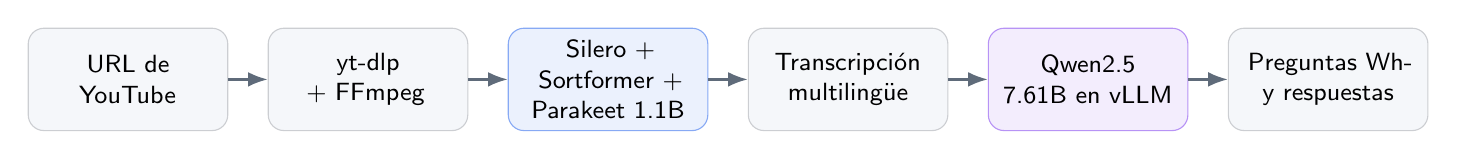
\begin{tikzpicture}[
    node distance=5mm,
    box/.style={draw=YTwoInk!22, rounded corners=2mm, minimum height=13mm,
      text width=23mm, align=center, fill=YTwoPaper, font=\sffamily\small},
    engine/.style={box, fill=YTwoBlue!9, draw=YTwoBlue!55},
    model/.style={box, fill=YTwoPurple!9, draw=YTwoPurple!55},
    arrow/.style={-{Latex[length=2.5mm]}, line width=0.8pt, draw=YTwoMuted}
  ]
    \node[box] (url) {URL de\\YouTube};
    \node[box, right=of url] (media) {yt-dlp\\+ FFmpeg};
    \node[engine, right=of media] (asr) {Silero +\\Sortformer +\\Parakeet 1.1B};
    \node[box, right=of asr] (text) {Transcripción\\multilingüe};
    \node[model, right=of text] (llm) {Qwen2.5\\7.61B en vLLM};
    \node[box, right=of llm] (qa) {Preguntas Wh-\\y respuestas};
    \draw[arrow] (url) -- (media);
    \draw[arrow] (media) -- (asr);
    \draw[arrow] (asr) -- (text);
    \draw[arrow] (text) -- (llm);
    \draw[arrow] (llm) -- (qa);
  \end{tikzpicture}
  }
  \caption{Pipeline local desde el video hasta el material de estudio.}
  \label{fig:local-pipeline}
\end{figure}

\begin{table}[htbp]
  \centering
  \caption{Modelos principales desplegados en la GB10.}
  \label{tab:deployed-models}
  \begin{tabularx}{\textwidth}{@{}l l r l X@{}}
    \toprule
    Etapa & Modelo & Parámetros & Precisión & Responsabilidad \\
    \midrule
    Voz a texto & Parakeet RNNT Multilingual & 1.1B & FP16 &
      Reconocimiento de voz en 25 idiomas y variantes. \\
    Texto a conocimiento & Qwen2.5-7B-Instruct & 7.61B & BF16 &
      Generación estructurada de preguntas Wh- y respuestas. \\
    \bottomrule
  \end{tabularx}
\end{table}

\section{Anatomía de Qwen2.5-7B-Instruct}

Qwen2.5-7B-Instruct es un Transformer \emph{decoder-only}. Su configuración
publicada especifica 28 bloques, dimensión oculta de 3,584, dimensión intermedia
de 18,944, 28 cabezas de consulta, cuatro cabezas Key/Value y vocabulario de
152,064 tokens. La variante cargada por vLLM usa BF16 y un contexto operativo de
32,768 tokens.

\begin{figure}[htbp]
  \centering
  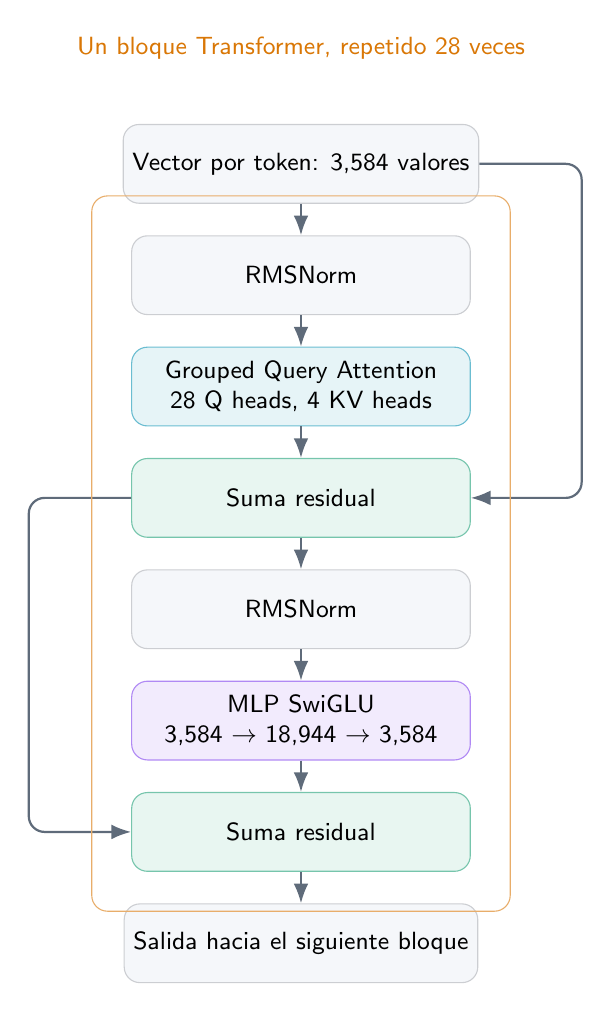
\begin{tikzpicture}[
    node distance=4mm,
    flow/.style={-{Latex[length=2.5mm]}, line width=0.8pt, draw=YTwoMuted},
    op/.style={draw=YTwoInk!22, rounded corners=2mm, minimum width=43mm,
      minimum height=10mm, align=center, fill=YTwoPaper, font=\sffamily\small},
    attn/.style={op, fill=YTwoCyan!10, draw=YTwoCyan!60},
    mlp/.style={op, fill=YTwoPurple!10, draw=YTwoPurple!60},
    residual/.style={op, fill=YTwoGreen!9, draw=YTwoGreen!55}
  ]
    \node[op] (input) {Vector por token: 3,584 valores};
    \node[op, below=of input] (norm1) {RMSNorm};
    \node[attn, below=of norm1] (attention) {Grouped Query Attention\\28 Q heads, 4 KV heads};
    \node[residual, below=of attention] (res1) {Suma residual};
    \node[op, below=of res1] (norm2) {RMSNorm};
    \node[mlp, below=of norm2] (ffn) {MLP SwiGLU\\3,584 $\rightarrow$ 18,944 $\rightarrow$ 3,584};
    \node[residual, below=of ffn] (res2) {Suma residual};
    \node[op, below=of res2] (output) {Salida hacia el siguiente bloque};

    \draw[flow] (input) -- (norm1);
    \draw[flow] (norm1) -- (attention);
    \draw[flow] (attention) -- (res1);
    \draw[flow] (res1) -- (norm2);
    \draw[flow] (norm2) -- (ffn);
    \draw[flow] (ffn) -- (res2);
    \draw[flow] (res2) -- (output);
    \draw[flow, rounded corners=2mm] (input.east) -- ++(13mm,0) |- (res1.east);
    \draw[flow, rounded corners=2mm] (res1.west) -- ++(-13mm,0) |- (res2.west);

    \node[draw=YTwoAmber!60, rounded corners=2mm,
      fit=(norm1)(attention)(res1)(norm2)(ffn)(res2), inner sep=5mm] {};
    \node[font=\sffamily\small, text=YTwoAmber, above=7mm of input]
      {Un bloque Transformer, repetido 28 veces};
  \end{tikzpicture}
  \caption{Flujo interno simplificado de un bloque Qwen2.5.}
  \label{fig:qwen-block}
\end{figure}

La atención relaciona posiciones de la transcripción. La MLP transforma cada
posición de manera no lineal y concentra la mayor parte de los parámetros. El
conocimiento no está guardado como registros independientes: emerge de patrones
distribuidos entre estas matrices.

\section{Distribución de parámetros y pesos}

Cada parámetro BF16 ocupa dos bytes. Por ello, 7.6156 mil millones de parámetros
requieren cerca de 15.23 GB decimales, o 14.19 GiB, antes de activaciones y
cachés de inferencia.

\begin{figure}[htbp]
  \centering
  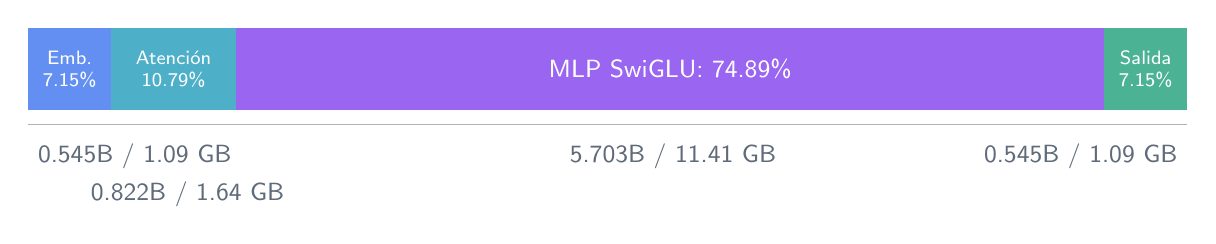
\begin{tikzpicture}[x=0.92cm,y=1cm,font=\sffamily\small]
    \def\W{16}
    \fill[YTwoBlue!72] (0,0) rectangle (1.144,1.05);
    \fill[YTwoCyan!72] (1.144,0) rectangle (2.870,1.05);
    \fill[YTwoPurple!78] (2.870,0) rectangle (14.854,1.05);
    \fill[YTwoGreen!72] (14.854,0) rectangle (16,1.05);
    \node[white, align=center, font=\sffamily\scriptsize] at (0.572,0.525) {Emb.\\7.15\%};
    \node[white, align=center, font=\sffamily\scriptsize] at (2.007,0.525) {Atención\\10.79\%};
    \node[white, align=center] at (8.862,0.525) {MLP SwiGLU: 74.89\%};
    \node[white, align=center, font=\sffamily\scriptsize] at (15.427,0.525) {Salida\\7.15\%};

    \draw[YTwoInk!35] (0,-0.18) -- (16,-0.18);
    \node[anchor=north west, text=YTwoMuted] at (0,-0.30)
      {0.545B / 1.09 GB};
    \node[anchor=north, text=YTwoMuted] at (2.2,-0.78)
      {0.822B / 1.64 GB};
    \node[anchor=north, text=YTwoMuted] at (8.9,-0.30)
      {5.703B / 11.41 GB};
    \node[anchor=north east, text=YTwoMuted] at (16,-0.30)
      {0.545B / 1.09 GB};
  \end{tikzpicture}
  \caption{Distribución aproximada de los 7.61B parámetros de Qwen2.5-7B-Instruct.}
  \label{fig:qwen-weights}
\end{figure}

\begin{table}[htbp]
  \centering
  \caption{Cálculo de parámetros principales.}
  \label{tab:qwen-parameter-math}
  \begin{tabularx}{\textwidth}{@{}l X r r@{}}
    \toprule
    Componente & Forma conceptual & Parámetros & BF16 aprox. \\
    \midrule
    Embedding & $152{,}064 \times 3{,}584$ & 0.545B & 1.09 GB \\
    Atención, 28 capas & Q, K, V y proyección de salida & 0.822B & 1.64 GB \\
    MLP, 28 capas & Gate, Up y Down & 5.703B & 11.41 GB \\
    Cabeza de salida & $3{,}584 \times 152{,}064$ & 0.545B & 1.09 GB \\
    \midrule
    Total & Incluye normas y sesgos menores & 7.616B & 15.23 GB \\
    \bottomrule
  \end{tabularx}
\end{table}

Un bloque contiene alrededor de 29.4M parámetros de atención y 203.7M de MLP,
para un total cercano a 233.1M. Los 28 bloques reúnen aproximadamente 6.53B
parámetros. La tabla de embeddings y la cabeza de salida no comparten pesos en
esta configuración.

\section{Memoria durante la inferencia}

Los pesos son sólo una parte del uso de memoria. vLLM también mantiene
activaciones temporales, áreas de trabajo CUDA, grafos compilados y la caché KV.
Esta última evita recalcular Keys y Values de todos los tokens anteriores cuando
el modelo genera el siguiente token.

Con cuatro cabezas KV, dimensión de cabeza 128, 28 capas y BF16, el coste ideal
por token es aproximadamente:

\begin{equation}
  2\;\text{(K,V)} \times 4\;\text{cabezas} \times 128 \times
  28\;\text{capas} \times 2\;\text{bytes}
  = 57{,}344\;\text{bytes/token}.
\end{equation}

Una secuencia de 32,768 tokens requiere cerca de 1.88 GB decimales de KV antes
de considerar concurrencia y alineamientos internos. Grouped Query Attention
reduce esta cifra porque 28 cabezas Query comparten sólo cuatro grupos KV.

\begin{figure}[htbp]
  \centering
  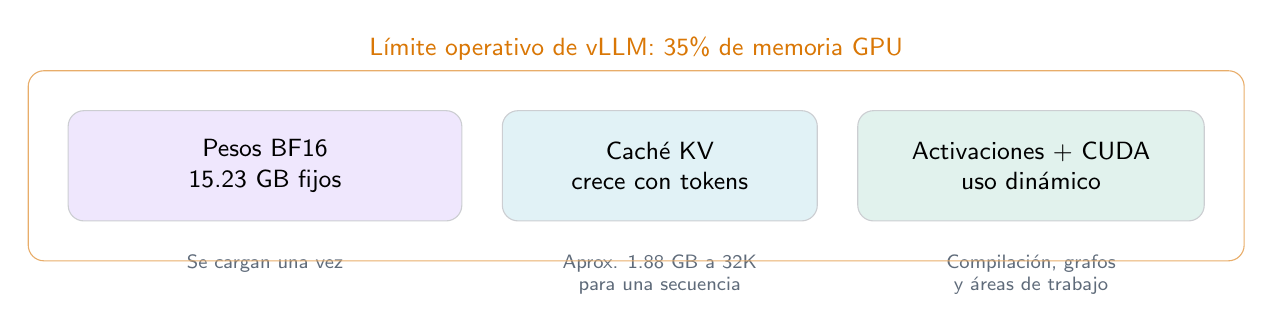
\begin{tikzpicture}[
    mem/.style={rounded corners=2mm, minimum height=14mm, align=center,
      font=\sffamily\small, draw=YTwoInk!22},
    note/.style={font=\sffamily\scriptsize, text=YTwoMuted, align=center}
  ]
    \node[mem, fill=YTwoPurple!12, minimum width=50mm] (weights)
      {Pesos BF16\\15.23 GB fijos};
    \node[mem, fill=YTwoCyan!12, minimum width=40mm, right=5mm of weights] (kv)
      {Caché KV\\crece con tokens};
    \node[mem, fill=YTwoGreen!12, minimum width=44mm, right=5mm of kv] (runtime)
      {Activaciones + CUDA\\uso dinámico};
    \node[note, below=3mm of weights] {Se cargan una vez};
    \node[note, below=3mm of kv] {Aprox. 1.88 GB a 32K\\para una secuencia};
    \node[note, below=3mm of runtime] {Compilación, grafos\\y áreas de trabajo};
    \node[draw=YTwoAmber!60, rounded corners=2mm,
      fit=(weights)(kv)(runtime), inner sep=5mm,
      label={[font=\sffamily\small, text=YTwoAmber]above:Límite operativo de vLLM: 35\% de memoria GPU}] {};
  \end{tikzpicture}
  \caption{Categorías de memoria del servicio LLM. El límite es un techo, no un consumo constante.}
  \label{fig:runtime-memory}
\end{figure}

\section{Estado de validación}

La cadena de modelos alcanzó los siguientes hitos en la DGX Spark GB10:

\begin{itemize}
  \item Parakeet respondió correctamente a una transcripción de muestra por la API HTTP de NVIDIA NIM.
  \item El perfil NIM seleccionado corresponde a DGX Spark, FP16, modo offline multilingüe, VAD Silero y diarización Sortformer.
  \item Qwen2.5-7B-Instruct se cargó en BF16 con FlashAttention 2 mediante vLLM 0.28.0.
  \item El servidor vLLM informó \texttt{Application startup complete} y respondió \texttt{200 OK} en \texttt{/health}.
  \item Los puertos de ASR y LLM permanecen enlazados a loopback; FastAPI actúa como orquestador local.
\end{itemize}

\section{Fuentes técnicas}

{\small NVIDIA,
\href{https://build.nvidia.com/nvidia/parakeet-1_1b-rnnt-multilingual-asr/modelcard}{Parakeet 1.1B RNNT Multilingual ASR Model Card};
Qwen Team,
\href{https://huggingface.co/Qwen/Qwen2.5-7B-Instruct}{Qwen2.5-7B-Instruct Model Card};
y Qwen Team,
\href{https://huggingface.co/Qwen/Qwen2.5-7B-Instruct/raw/main/config.json}{Qwen2.5-7B-Instruct configuration}.}

\end{document}
